\documentclass[10pt,xcolor={svgnames}]{beamer}

%%%%% Colors
\usetheme{Dresden}%\usetheme{Madrid}
\colorlet{beamer@blendedblue}{green!55!black}
%%%%%

%%%%% Other 
\addtobeamertemplate{navigation symbols}{}{%
    \usebeamerfont{footline}%
    \usebeamercolor[fg]{footline}%
    \hspace{1em}%
    \insertframenumber/\inserttotalframenumber
}
\usepackage{hyperref, url}

\definecolor{pine_green}{HTML}{007935}
\hypersetup{colorlinks,breaklinks,linkcolor=white,urlcolor=orange,citecolor=black}
\renewcommand\thefootnote{\textcolor{pine_green}{\arabic{footnote}}}
\setbeamercolor{alerted text}{fg=pine_green}

\usepackage{cancel}
\usepackage{ulem}
\usepackage{multirow}
\usepackage{mathtools}
\setbeamertemplate{itemize subitem}{$\circ$}

%https://tex.stackexchange.com/questions/289542/auto-resizing-parenthesis-in-math-formulas
% \usepackage{amsmath} for testing
\newcommand*\autoop{\left(}
\newcommand*\autocp{\right)}
\newcommand*\autoob{\left[}
\newcommand*\autocb{\right]}
\AtBeginDocument {%
   \mathcode`( 32768
   \mathcode`) 32768
   \mathcode`[ 32768
   \mathcode`] 32768
   \begingroup
       \lccode`\~`(
       \lowercase{%
   \endgroup
       \let~\autoop
   }\begingroup
       \lccode`\~`)
       \lowercase{%
   \endgroup
       \let~\autocp
   }\begingroup
       \lccode`\~`[
       \lowercase{%
   \endgroup
       \let~\autoob
   }\begingroup
       \lccode`\~`]
       \lowercase{%
   \endgroup
       \let~\autocb
   }}

\delimiterfactor 1001

\makeatletter
% for amsmath "compatibility" (not sophisticated)
% \usepackage{amsmath}
\AtBeginDocument {%
          \def\resetMathstrut@{%
           \setbox\z@\hbox{\the\textfont\symoperators\char40}%
           \ht\Mathstrutbox@\ht\z@ \dp\Mathstrutbox@\dp\z@}%
}%
\makeatother
%%%%%

%%%%% Greying out/invidible Slides
\setbeamercovered{invisible}
\setbeamercovered{%
  again covered={\opaqueness<1->{15}}}
  
%%%%%







%%%%% Footnotes and captions
%\usepackage[utf8]{inputenc}
\usepackage{caption}
\usepackage{comment}
\usepackage{wasysym}
\setbeamerfont{footnote}{size=\tiny}
\setbeamerfont{caption}{size=\tiny}
%\setbeamerfont{normal text}{size=\small}
\setbeamerfont{itemize/enumerate body}{size=\small}
\setbeamerfont{itemize/enumerate subbody}{size=\footnotesize}
%%%%%



%Information to be included in the title page:
\title[Connor Wiegand]{Intro to Economic Analysis: Microeconomics}
\subtitle{EC 201 - Day 4 Slides}
\author[EC 201]{Connor Wiegand}
\institute[]{Department of Economics - University of Oregon}
\date{6 October 2021}


\begin{document}

\frame{\titlepage}

\begin{frame}{Logistics}
    \begin{itemize}[<+->]
        \item Official homework 1 due this Saturday at 11:59pm, covering last week's material
        \item News assignments posted, first one due Wednesday, October 13
        \begin{itemize}
            \item This includes doing 1 news analysis of your choice on Cengage, \underline{and}
            \item Submitting a 1-1.5 page write up on Canvas
        \end{itemize}
        \item The outline must contain a brief summary of the article you read, as well as responses to the discussion questions that were at the end of your Cengage News Analysis    
        \end{itemize}
\end{frame}

\begin{frame}{The Relationship Between Price and Quantity, As a Producer}
    \begin{itemize}[<+->]
        \item Previously, we explored as consumers how much of a good you would consume at a specific price
        \item For producers, one could imagine the same thought experiment: how many iced coffees would I sell for a specific price
        \item However, much like we faced carrying constraints as consumers, we face storage and cost constraints as producers
        \begin{itemize}
            \item Say it costs you \$2 to make an iced coffee with the supplies you have on hand
            \item Coffee goes for \$3, so you would like to sell infinite iced coffees
            \item However, once you make 10 gallons of iced coffee, you have run out of fridge space, so you have to incur the cost of a new fridge
            \item And shortly thereafter, you have to buy more storage for your coffee beans, and then more laborers to make iced coffee, so on and so forth
            \item All of these things affect your cost of making an iced coffee
        \end{itemize}
        \item Later in the course, we will explore in more detail how these cost structures generate a supply curve  
    \end{itemize}
\end{frame}

\begin{frame}{The Relationship Between Price and Quantity, As a Producer}
    \begin{itemize}[<+->]
        \item For now, we will simply take as given that these structures influence the following supply schedule \textit{for a producer}:
        \begin{table}[H]
            \centering
            \begin{tabular}{c|c}
                Price & Quantity Supplied \\
                \hline
                \$0 & 0\\
                \$1 & 2\\
                \$2 & 3\\
                \$3 & 4\\
                \$4 & 4.5\\
                \$5 & 5
            \end{tabular}
        \end{table}
    \end{itemize}
\end{frame}


\begin{frame}{Individual Supply Curve}
    \begin{itemize}
        \item This set of points can be used to establish the producer's \underline{individual supply curve}
        \begin{center}
            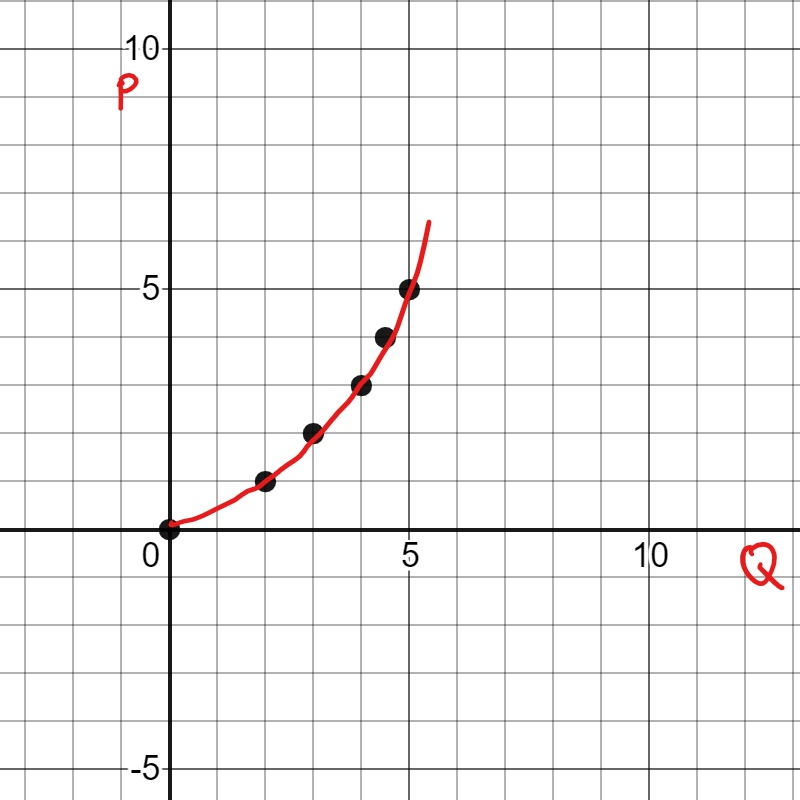
\includegraphics[width=5cm]{desmos indi supply.jpg}
        \end{center}
        \item Once again, the exact reasoning for the shape of this curve is motivated by possible cost structure: the producer may have to incur high costs of their own just to produce 5 coffees (say, per 15 minutes)
    \end{itemize}
\end{frame}

\begin{frame}{Market Supply}
    \begin{itemize}[<+->]
        \item Just as before, we can take their \underline{horizontal sum} of individual supply curves to get market supply
        \begin{itemize}
            \item That is, if the market consists of 3 producers, who each supply $q_{1}$, $q_{2}$, and $q_{3}$ iced coffees at a price of \$1, then the market supply for iced coffee at \$1 is $Q_{M}=q_{1}+q_{2}+q_{3}$
            \begin{center}
                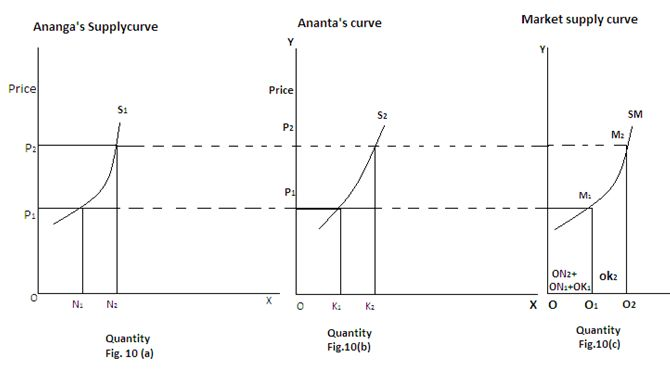
\includegraphics[width=8cm]{summing supply.jpg}
            \end{center}
        \end{itemize}
    \end{itemize}
\end{frame}

\begin{frame}{Market Supply Simulation}
    \begin{itemize}[<+->]
        \item For example, if I am one supplier in the economy, and I have two of you as members of the economy, so that our three individual supply curves look like the this (left):
        \begin{table}[H]
            \centering
            \begin{tabular}{ll}
                \hspace{-18mm}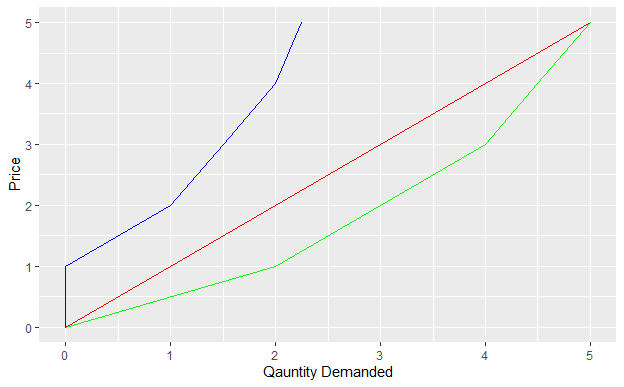
\includegraphics[width=6cm]{3 indi supply.png} & \pause 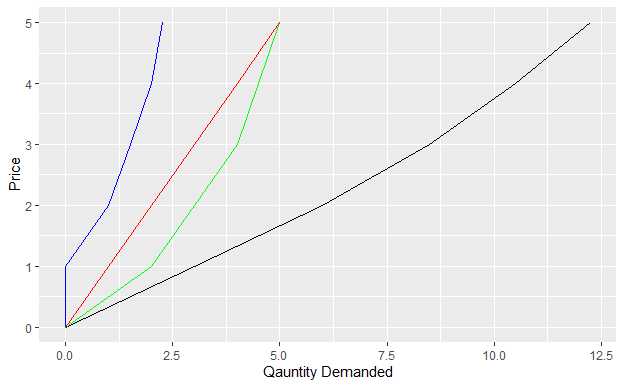
\includegraphics[width=6cm]{market simulation supply.png}  
            \end{tabular}
        \end{table}
        \item Then our market supply will look like this (right)
    \end{itemize}
\end{frame}

\begin{frame}{Supply Curve Features}
    \begin{itemize}[<+->]
        \item What is the most obvious feature of the supply curve? 
        \begin{itemize}
            \item It's upward sloping
        \end{itemize}
        \item This says that the relationship between price and quantity demanded is positive: as the price goes up, you (or the market) generally are willing to supply more of the good in question
        \item This is formally known as the \underline{\textbf{Law of Supply}}: ``Other things being equal, when the price of a good rises, the quantity supplied of the good also rises, and when the price falls, the quantity supplied falls as well"
    \end{itemize}
\end{frame}

\begin{frame}{Specificity of Market}
\begin{itemize}[<+->]
    \item Note that the supply curve measures the supply for a good in the \textit{market}, a key feature of microeconomics
    \item However, we can of course seek out various levels of specificity when defining these goods
    \item Ex: 
    \item Each time we move to a different tier, we may expect different characteristics in the shape of the supply curve
    \item We may also expect general trends as we move to more specific levels, which is a topic for next chapter
    \item Economists will often not compare supply curves across these different tiers, but it is not out the question (for example, when studying a specific firm with few types of services, like Uber)
\end{itemize}
\end{frame}

\begin{frame}{Other Features of the Supply Curve}
    \begin{itemize}[<+->]
        \item Just as before, we can define specificity of the market for the good in question, for example: Medicine \& Prescription Medication $>$ Opiods $>$ Percocet $>$ Brand-name Percocet
        \item The shape of the supply curve is usually draw either like and exponentional or linear, but again this is usually not of huge concern
        \item While the slope of the supply curve is of great importance, and we will discuss further in the next chapter and beyond
        \item The biggest topic in this chapter relating to the supply curve will being shifting it, or moving along it
    \end{itemize}
\end{frame}

\begin{frame}{What Would Cause Market Supply Curve to Shift?}
    \begin{itemize}[<+->]
        \item Changes in...
        \item Prices of inputs
        \begin{itemize}
            \item If the price of sugar falls, the supply of candy will rise
        \end{itemize}
        \item Technology
        \begin{itemize}
            \item If you find a way to produce 2x the vaccines in a given period of time, the supply of vaccines will rise
            \item If a natural disaster wipes out all of the corn in the midwest, the supply of whiskey will fall \footnote{This could be a shift due to technology getting worse, or due to input prices rising}
        \end{itemize}
        \item Number of sellers in the market
        \begin{itemize}
            \item If a bunch of people think they can get rich through \sout{Pyramid Schemes} MLM businesses, the supply of skincare products is likely to rise
        \end{itemize}
        \item Expectations
        \begin{itemize}
            \item The green paradox: some environmental policies can do harm by announcing higher taxes in the future
            \item Ex: If we say that we will heavily tax producers for extracting oil 1 year from now, they will likely extract more today and in the next 364 days
        \end{itemize}
    \end{itemize}
\end{frame}

\begin{frame}{Changes in Price}
    \begin{itemize}
        \item So our shifters of supply are
        \begin{itemize}
            \item changes in price of inputs
            \item changes in technology
            \item changes in \# of sellers in the market
            \item changes in expectations
            \item And natural disasters
        \end{itemize}
        \item<2-> Once again, changes in the the price of good $x$ only lead to a movement along the supply curve, rather than a shift in the curve
        \item The reasoning is the same as last time
    \end{itemize}
\end{frame}

\begin{frame}{What Do These supply Changes Look Like?}
    \begin{itemize}[<+->]
        \item When supply rises, we say that the supply curve shifts \underline{to the right} (rightward)
        \item When supply falls, we say that the supply curve shifts \underline{to the left} (leftward)
        \item Why the difference compared to demand? 
        \begin{enumerate}
            \item Since demand slopes downward, it often creates a closed region in the positive quadrant, so shifting in/out makes sense. This does not happen with supply
            \item Additionally, with supply, an shift downward in the $b$ value of $y=mx+b$ actually corresponds to an \textit{increase} in supply. Again, this is due to supply being upward sloping: imagine a curve starting at the origin sloping up. If we 
        \end{enumerate}
        \item We also may just say that supply rises or falls\footnote{\vspace{2mm}On a test or assignment, you should be \underline{very} clear on whether or not you mean a curve shift or a movement along the curve}
    \end{itemize}
\end{frame}

\begin{frame}{Visualizing Changes in Price}
    \begin{itemize}
        \item Suppose I gave you the equation $y=mx+b$, for instance, $y=2x+4$
        \item A shift in supply is akin to changing the value of $b$, say from $b=4$ to $b=1$:
        \begin{center}
            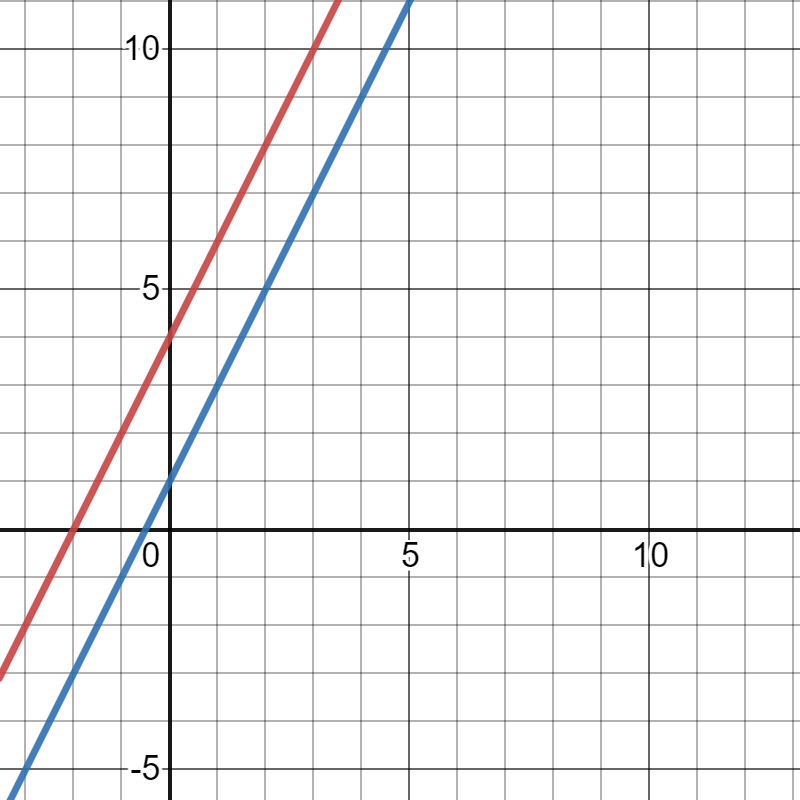
\includegraphics[width=4cm]{desmos supply shift.png}
        \end{center}
        \item Again, notice that the quantity supplied at $P=\$4$ (using $P$ instead of $y$) rises from 0 to 1.5 on the graph
    \end{itemize}
\end{frame}

\begin{frame}{Changes in Price (cont.)}
    \begin{itemize}[<+->]
        \item However, suppose that I instead said that $y$ changed from $6$ to $8$. How do I move the curve?
        \item A: I don't. If $y=6$, then I know that we are at the point $(1,6)$ on the curve. If the $y$ value rose to $8$, then I just move along the curve to $(2,8)$
        \begin{center}
            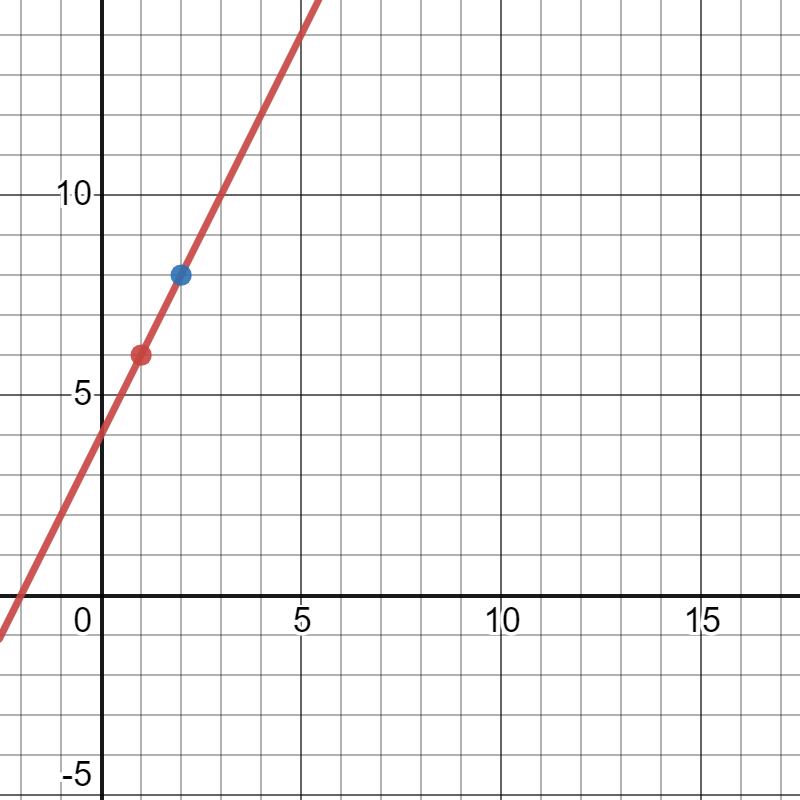
\includegraphics[width=4cm]{desmos supply move.png}
        \end{center}
    \end{itemize}
\end{frame}

\begin{frame}{Summary of Supply Shifts}
    \begin{center}
        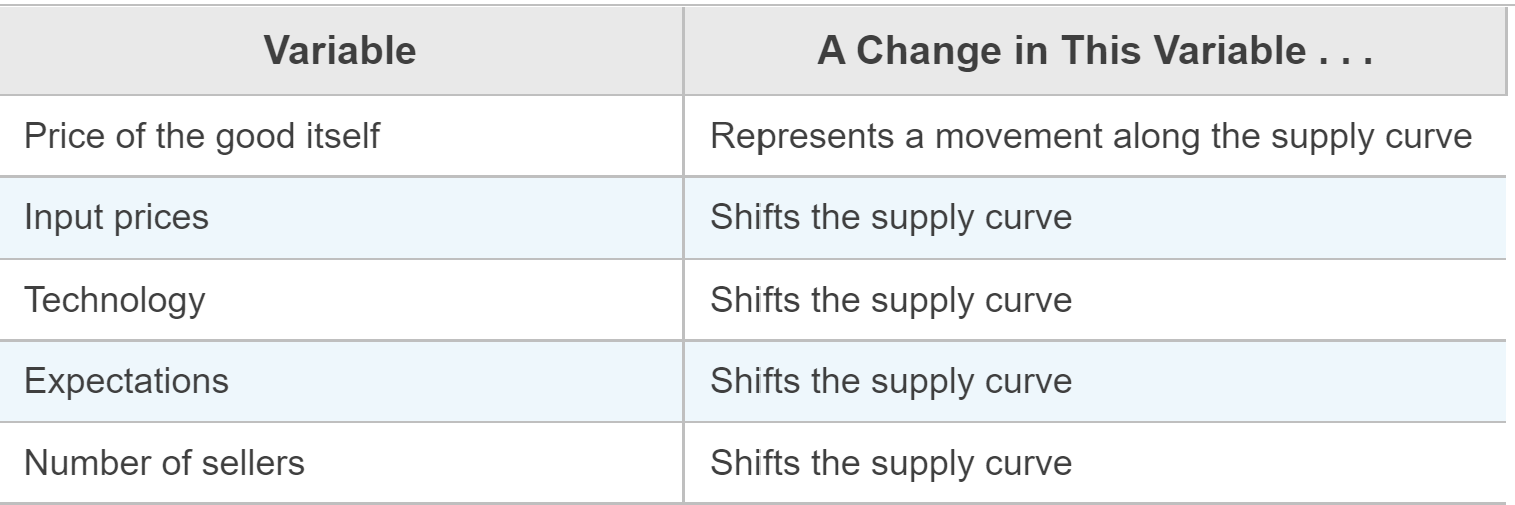
\includegraphics[width=7cm]{summary supply shift.png}
    \end{center}
    \begin{itemize}
        \item When supply shifts, it is best to say that ``the supply curve shifts" or that ``supply shifts"
        \item When there is a movement along the curve, it you should make this clear by saying something to the effect of a ``movement along the supply curve", or you can say that quantity demanded goes up or down (but you should make clear that you mean a movement not a curve shift)
        \item In short, do not say in either case that ``supply moves", be clear about what you mean, and use the terminology presented; otherwise I will assume you do not know what you are talking about
    \end{itemize}
\end{frame}

\begin{frame}{Combining the Curves}
    \begin{itemize}
        \item As one might imagine, we are now going to combine the supply and demand curves
        \item When we graph supply and demand together, their intersection is known as \underline{\textbf{market equilibrium}}
        \item In this case, the price at which the curves intersect is called \underline{\textbf{equilibrium price}} (or \textit{market price)} and the common point where quantity supplied equals quantity demanded (that is, the quantity where the curves intersect) is the \underline{\textbf{equilibrium quantity}}
        \begin{itemize}
            \item Generally, equilibrium objects are denoted: $P^{*}$, $P_{e}$, $P^{E}$ 
            \item When considering more than one equilibrium, you may write $P_{0}$ or $P_{1}$ for the initial equilibrium, and then index up by 1, or you may write $P$ and add primes, i.e. $P'$, $P''$, etc. Just make sure it is clear to your grader that you understand the concept
        \end{itemize}
        \item When the market is in equilibrium, it is also said that the market \textit{clears}, and the former  instances of `equilibrium' are replaced with `market clearing'
    \end{itemize}
\end{frame}

\begin{frame}{Market Equilibrium}
    \begin{itemize}
        \item ``At the equilibrium price, the quantity of the good that buyers are willing and able to buy exactly balances the quantity that sellers are willing and able to sell" -- Mankiw
        \begin{center}
            \hspace{-15mm}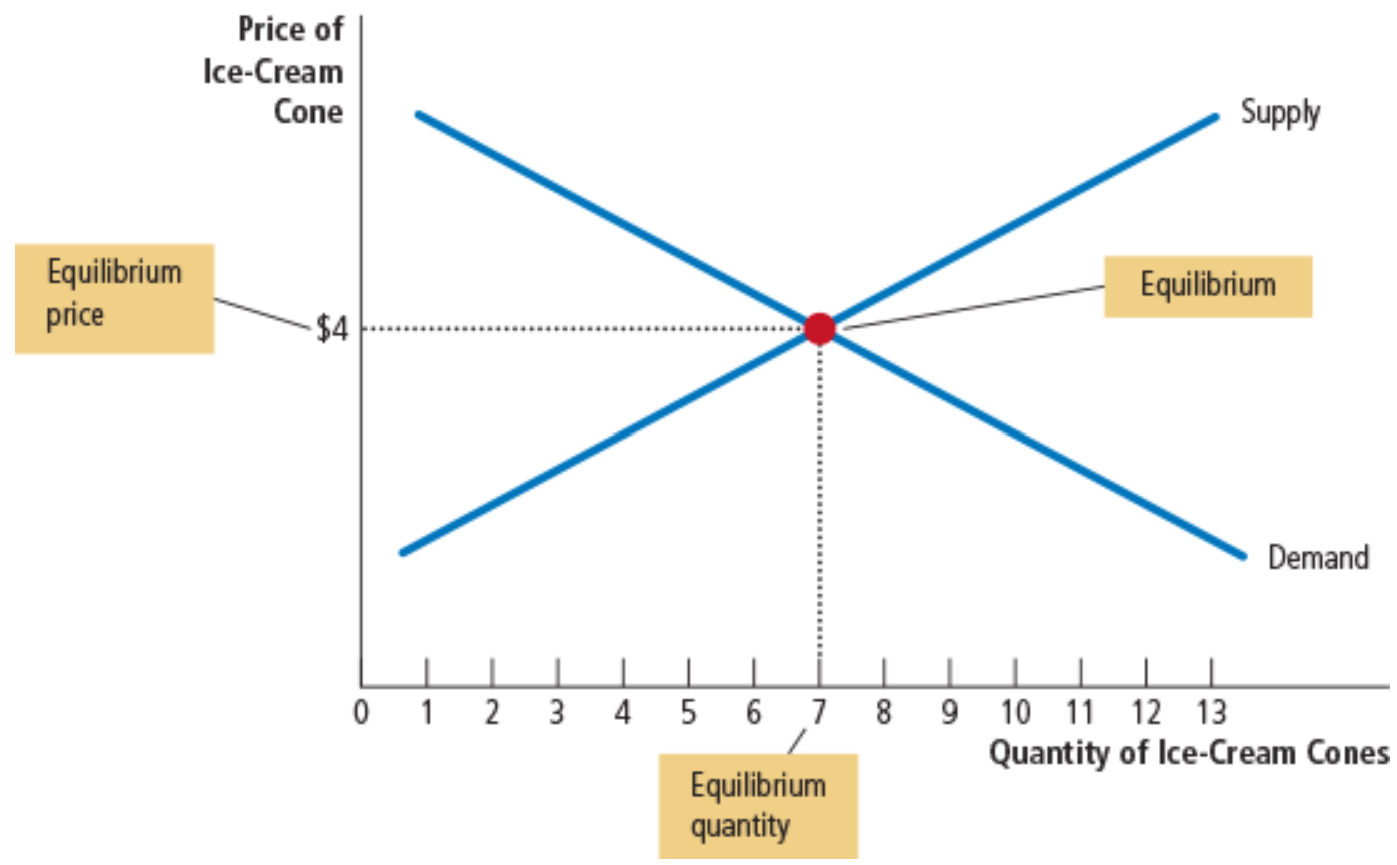
\includegraphics[width=6cm]{market equilibrium.png}
        \end{center}
        \item If you report the equilibrium as a point, make sure to indicate which is $P$ and which is $Q$\footnote{\vspace{1.5mm}Usually, points are recorded $(x,y)$, but equilibria are often recorded at $(P^{*},Q^{*})$, so just make it clear}
        \begin{itemize}
            \item E.g. $(P^{*},Q^{*})=(4,7)$
        \end{itemize}
    \end{itemize}
\end{frame}

\begin{frame}{Market Dis-equilibrium}
    \begin{itemize}[<+->]
        \item Don't get stuck on what's visually appealing: we can instigate that a market is in dis-equilibrium
        \item We may say that the price of ice cream is \$5 in the above figure, and ask you to solve for $Q_{d}$ and $Q_{s}$
        \item However, we generally believe as economists (and in this model) that the market will corrects itself, by moving along each curve back to the equilibrium
    \end{itemize}
\end{frame}

\begin{frame}{Market Dis-equilibrium (cont.)}
    \begin{itemize}
        \item This is covered in more detail in the book, as evidenced by the following picture. We will cover surpluses and shortages in finer detail in a later chapter 
        \begin{center}
            \hspace{-15mm}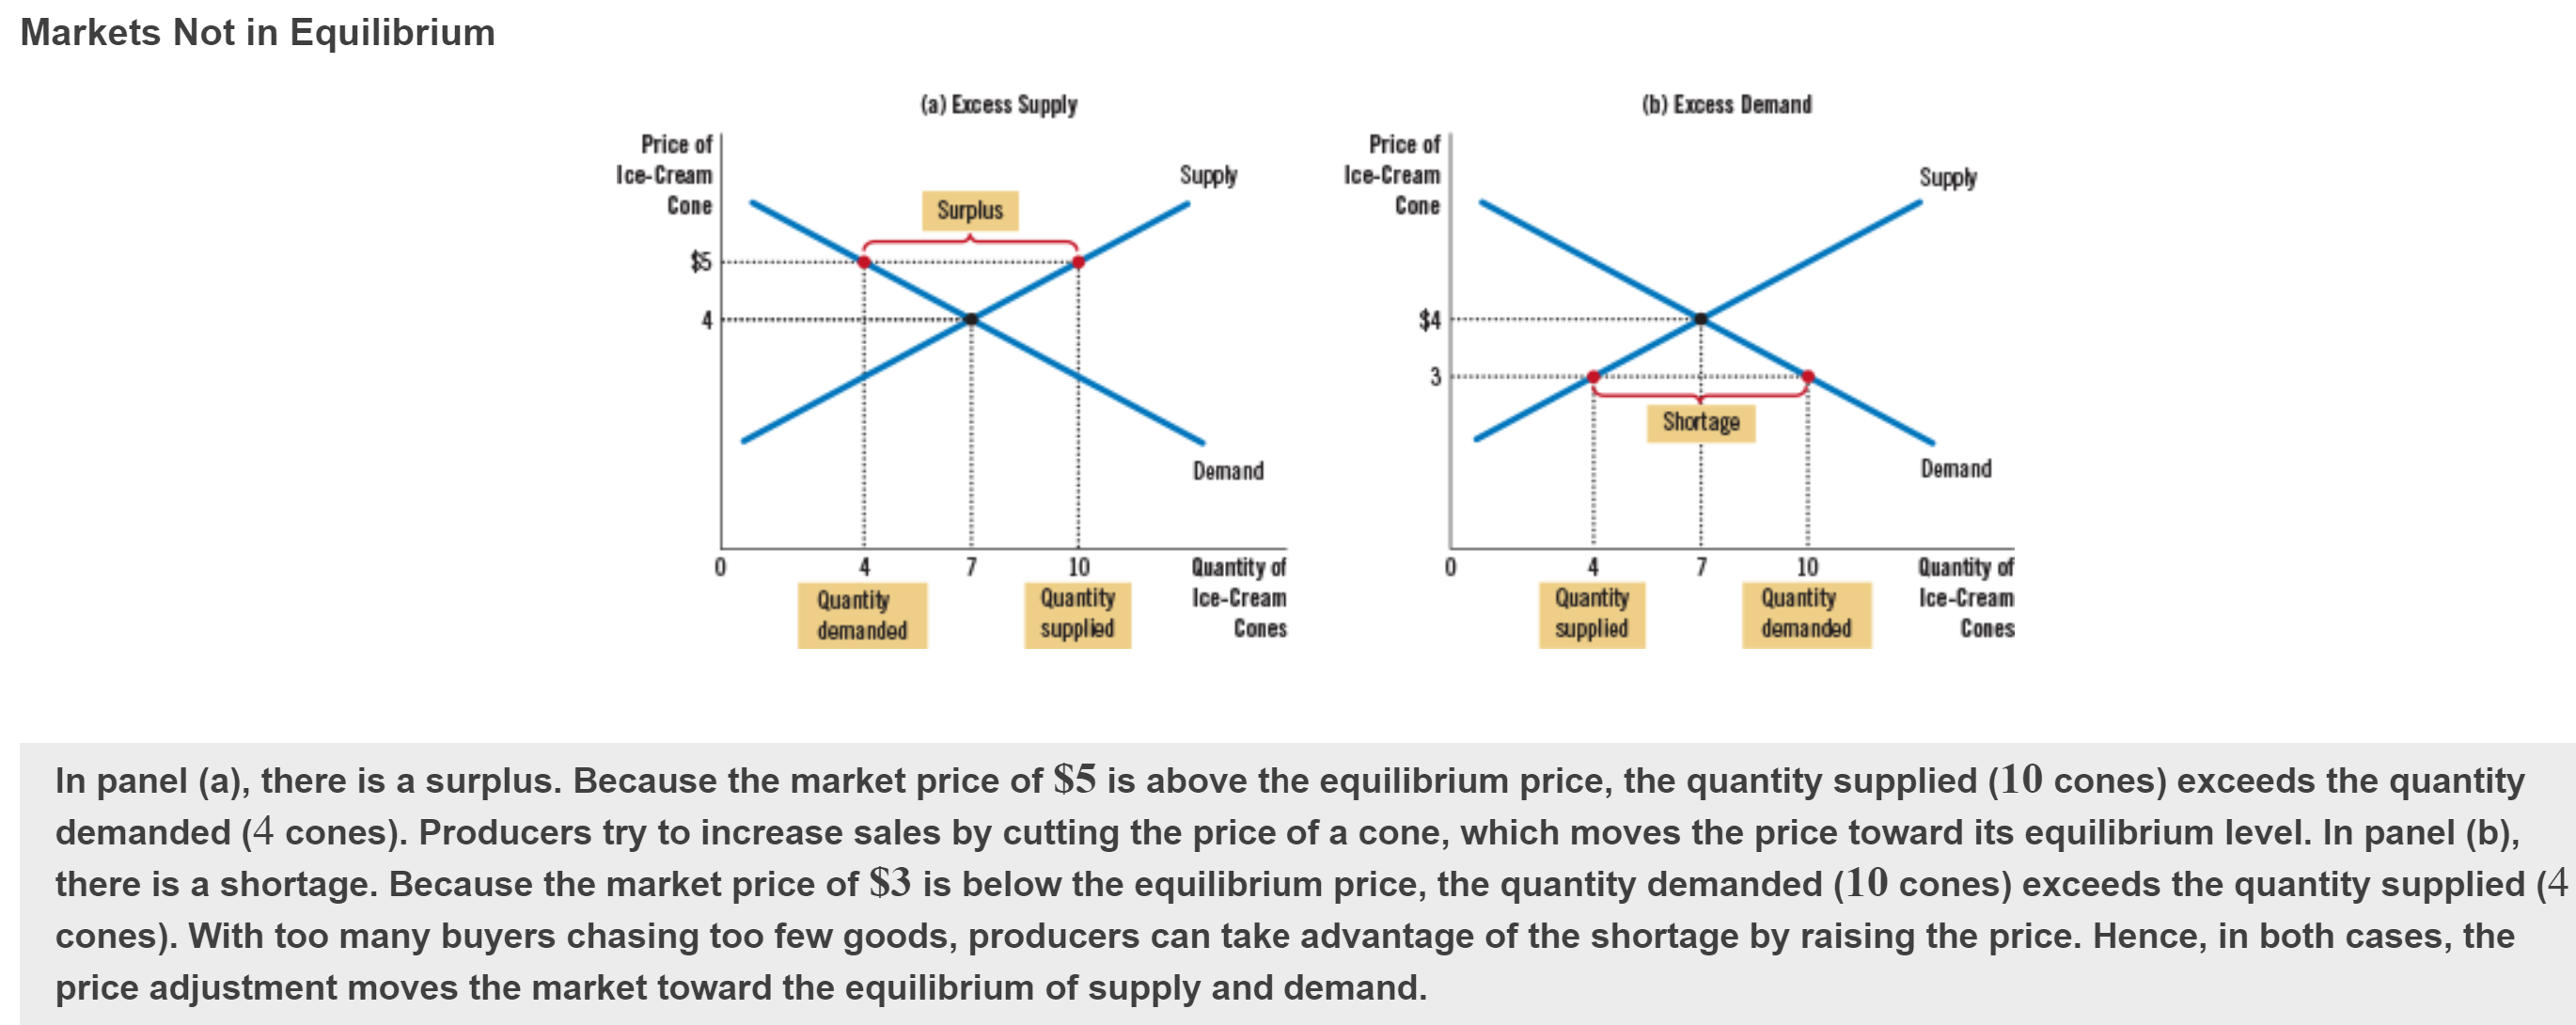
\includegraphics[width=11.5cm]{diseq.png}
        \end{center}
    \end{itemize}
\end{frame}

\begin{frame}{Math Review}
    \begin{itemize}
        \item By now, we have practiced a little algebra and graphing skills, and there was the intro refresher
        \item I want to formally cover some important mathematical concepts in detail 
        \item If you feel you need more practice, I would encourage seeking out resources online, or coming to office hours
        \begin{itemize}
            \item Kahn Academy is a good resources
            \item Paul's Online Math Notes are fantastic
            \item Purple Math, also just googling "algebra resources" or "algebra help" or something similar will pull up numerous great resources
        \end{itemize}
        \item Homework is also another form of practice
        \item What we will cover today is not necessarily comprehensive, and you should be familiar with everything that is in the algebra cheat sheet I posted online
    \end{itemize}
\end{frame}

\begin{frame}{Math Review -- Fractions}
    \begin{itemize}
        \item \underline{Consider the fraction} $\frac{a}{b}$
        \item $\frac{b}{a}$ is called the reciprocal, and is equal to $\frac{1}{a/b}$, or $(\frac{a}{b})^{-1}$
        \item $\frac{a}{b}\cdot c=\frac{a\cdot c}{b}$
        \item $\frac{a}{b}\div c = \frac{a}{b\cdot c}$
        \item $\frac{a}{b}\cdot\frac{c}{d}=\frac{a\cdot c}{b\cdot d}$
        \item Consequently, 
        $$\frac{a}{b}=\frac{a}{b}\cdot 1=\frac{a}{b}\cdot \frac{c}{c}=\frac{a\cdot c}{b\cdot c}$$
        \item To add fractions, they have to be of common denominator. When they have a common denominator, 
        $\frac{a}{b}+\frac{c}{b}=\frac{a+c}{b}$
        \item Examples of adding fractions:
        \begin{itemize}
            \item $\frac{1}{3}+\frac{1}{9}=\frac{3}{9}+\frac{1}{9}=\frac{4}{9}$
            \item $$\frac{6}{19}+\frac{4}{13}=\frac{6\cdot 13}{19\cdot 13}+\frac{4\cdot 19}{13 \cdot 19}=\frac{78}{247}+\frac{76}{247}=\frac{154}{247}$$
        \end{itemize}
    \end{itemize}
\end{frame}

\begin{frame}{Math Review -- Arithmetic and Algebra}
    \begin{itemize}
        \item $\sqrt[n]{a}=a^{1/n}$
        \item $\sqrt{\frac{a}{b}}=\frac{\sqrt{a}}{\sqrt{b}}$ and $\sqrt{ab}=\sqrt{a}\sqrt{b}$
        \item $a^{n}b^{n}=(ab)^{n}$, $a^{n}a^{m}=a^{n+m}$, and $(a^{n})^{m}=a^{n\cdot m}$
        \item $\frac{a^{n}}{b^{n}}=(\frac{a}{b})^{n}$ and $(\frac{a}{b})^{-n}=\frac{b^{n}}{a^{n}}$
        \item $a^{-n}=\frac{1}{a^{n}}$, $\frac{1}{a^{-n}}=a^{n}$, and $\frac{a^{n}}{a^{m}}=a^{n-m}$
        \item $(-x)^{2}=x^{2}$. Notice that $(-3)^{2}=9$ but $-(3^{2})=-9$
        \item If $ax^{2}+bx+c=0$, then the quadratic formula can be used to solve for $x$:
        $$x=\frac{-b\pm\sqrt{b^{2}-4ac}}{2a}$$
        Note that this will yield two values, and we will not use complex (imaginary) numbers in this class, so choose the value that makes sense\footnote{Unless specified otherwise, prices and quantities will not be negative}
    \end{itemize}
\end{frame}

\begin{frame}{Math Review -- Basic Algebra}
    \begin{itemize}
        \item Recall that dividing by a fraction is the same as multiplying by the reciprocal, e.g.
        $$\frac{5}{13}y=2x \implies y=\frac{13}{5}(2x)=\frac{26}{5}x$$
        \item In general, when solving a single equation for a variable, you should aim to get that variable by itself by performing the same action to both sides, e.g.
        \begin{align*}
            \frac{2}{3}&P+\frac{5}{6}Q=10\\
            \implies \frac{2}{3}&P=10-\frac{5}{6}Q\\
            \implies &P=10(\frac{3}{2})-(\frac{5}{6})(\frac{3}{2})Q\\
            \implies &P=\frac{30}{2}-\frac{15}{12}Q\\
             \implies \Aboxed{&P=15-\frac{5}{4}Q}
        \end{align*}
    \end{itemize}
\end{frame}

\begin{frame}{Math Review -- Solving Two Variable Systems of Equations}
    \begin{itemize}
        \item Suppose 
                \begin{align*}
            ax+by&=c\\
            sx+ty&=u
        \end{align*}
        Where $x$ and $y$ are variables, and the rest of the numbers are constants
        \item The two ways to solve for this are:
        \begin{enumerate}
            \item $[\text{Method of Substitution}]$: Solve one equation for one variable in terms of the other (i.e. $x$ in terms of $y$ or $y$ in terms of $x$). Then, plug whatever you solved for into the other equation, to solve for one variable. Plug this back in to solve for the other
            \item $[\text{Method of Elimination}]$: Get to a point where you can add/subtract some multiple of one equation to the other to eliminate one variable. Solve for this variable, and use one of the equations to back out the other
        \end{enumerate}
        \begin{itemize}
            \item Note that one ``version" of the method of substitution is just to solve both equations for one variable, then set them equal to each other to get one variable, and then use this to get the other. For instance, solve both equations for $x$ in terms of $y$, then set them equal to get one equation in terms of $y$. Solve for $y$ and use this and one of the equations for $x$ in terms of $y$ to get $x$ 
        \end{itemize}
    \end{itemize}
\end{frame}

\begin{frame}{Math Review -- Method of Substitution}
    \begin{itemize}[<+->]
        \item Example: \begin{align}
            2x+6y&=8\\
            x-2y&=15
        \end{align}
        \item Solve (2) for $x$ in terms of $y$: $x=2y+15$
        \item Plug into (1) for $x$: 
        $$2(2y+15)+6y=8$$
        \item Solve for $y$:
        \begin{align*}
            4&y+30+6y=8\\
            \implies 10&y=-22\\
            \implies &y=-\frac{22}{10}=-\frac{11}{5}
        \end{align*}
        \item Solve for $x$, using known $y$ and first step:
        $$x=2y+15=2(-\frac{11}{5})+15=-\frac{22}{5}+\frac{75}{5}=\frac{53}{5}$$
    \end{itemize}
\end{frame}

\begin{frame}{Math Review -- Method of Elimination}
    \begin{itemize}[<+->]
        \item Example: 
        \begin{align*}
            2x+6y&=8\tag{1}\\
            x-2y&=15\tag{2}
        \end{align*}
        \item Multiply (2) by $-2$ on either side:
        \begin{align}
            -2x+4y=-30
        \end{align}
        \item Add (3) to (1): 
        $$10y=-22$$
        \item Solve for $y$: $y=-\frac{22}{10}=-\frac{11}{5}$
        \item Solve for $x$, using known $y$ and equation (2):
        \begin{align*}
            x-2y=15 \implies x-2(-\frac{11}{5})=15&\implies x+\frac{22}{5}=15 \\
            &\implies x=\frac{75}{5}-\frac{22}{5}=\frac{53}{5}
        \end{align*}
    \end{itemize}
\end{frame}

\begin{frame}{Exercise 1}
    \begin{itemize}[<+->]
        \item Suppose supply and demand are given by 
        \begin{align*}
            S: 4P-Q-4=0\\
            D: P-18=-4Q
        \end{align*}
        Find the market equilibrium (note that this means to find equilibrium quantity and price)
    \end{itemize}
\end{frame}

\begin{frame}{Solution 1}
    \begin{itemize}
        \item I will rewrite the equations as
        \begin{align*}
            &S: P=\frac{1}{4}Q+1\\
            &D: P=-4Q+18
        \end{align*}
        \item Setting them equal, we get 
        \begin{align*}
            \frac{1}{4}Q+1=-4Q+18 &\implies Q(4+\frac{1}{4})=17\\
            &\implies Q(\frac{16}{4}+\frac{1}{4})=17 \implies Q(17/4)=17\\
            &\implies Q^{*}=4   
        \end{align*}
        Plugging this into demand, we get $P^{*}=2$ 
    \end{itemize}
\end{frame}


\begin{frame}{Exercise 2}
    \begin{itemize}[<+->]
        \item Suppose supply and demand are given by 
        \begin{align*}
            &S: (P-3)(Q-4)=1\\
            &D: \sqrt{P-3}=Q-4
        \end{align*}
        \item Find the market equilibrium
    \end{itemize}
\end{frame}

\begin{frame}{Solution 2}
    \begin{itemize}[<+->]
        \item Solve supply and demand for $P$ in terms of $Q$:
        \begin{align*}
            S: P=\frac{1}{Q-4}+3\qquad 
            D: P=(Q-4)^{2}+3
        \end{align*}
        \item Setting them equal:
        $$\frac{1}{Q-4}+3=(Q-4)^{2}+3$$
        \item Solving:
        \begin{align*}
            \frac{1}{Q-4}=(Q-4)^{2} &\implies 1=(Q-4)^{3}\implies 1^{1/3}=Q-4\\
            &\implies Q-4=1 &implies Q^{*}=5
        \end{align*}
        \item Plug into supply equation:
        $$P^{*}=\frac{1}{5-4}+3=1+3=4$$
    \end{itemize}
    \label{Sol2}
\end{frame}

\begin{frame}{Math Review -- Graphing}
    \begin{itemize}
        \item Recall that points of the form $(a,b)$ communicate that the $x$ value is $a$ and the $y$ value is $b$ on a graph
        \item To calculate the slope of a line which crosses through points $(x_{1}, y_{1})$ and $(x_{2},y_{2})$, you compute 
        $$s =\frac{y_{2}-y_{1}}{x_{2}-x_{1}}$$
        which is refereed to as rise over run. This means that the line moves up (or down, if $s$ is negative) $s$ for every 1 unit of $x$ moved
        \item If $y=f(x)$ is a function, then $y=f(x)+a$ is that same function, translated up (or down, if $a$ is negative) by $a$ units
        \item If $y=f(x)$ is a function, then $y=f(x-a)$ is that same function, translated right (or left, if $a$ is negative) by $a$ units (this should seem backwards, but it is correct)
    \end{itemize}
\end{frame}

\begin{frame}{Exercise 3}
    \begin{itemize}[<+->]
        \item Suppose demand for candy is given by $P=1/Q$. Upon buying any amount of candy, you are given 2 extra pieces (units) for free, which shifts demand right by 1. Additionally, the government gives you 3 dollars as a subsidy, whenever you buy candy; this shifts demand up by 3
        \item What is the new demand equation?
    \end{itemize}
\end{frame}

\begin{frame}{Solution 3}
    \begin{itemize}[<+->]
        \item Shifting right by 2 means we replace $Q$ with $Q-2$. Shifting up by $3$ means we add 3 at the end of the equation
        \item Our new demand equation is thus given by
        $$P=\frac{1}{Q-2}+3$$
        \item You might be wondering why getting a piece of candy means we subtract 2 from $Q$. Before, at \$1, we demanded 1 piece. Now, at \$1, we demand 3 pieces, 2 of which are given for free
        \item Also, note that subsidizing effectively subtracts \$3 from the price. Subtracting \$3 from $P$ in the demand equation, and then resolving for \$P in terms of \$Q, will yield a $+3$ on the other side
    \end{itemize}
    \label{Sol3}
\end{frame}

\begin{frame}{Math Review -- Graphing with Desmos}
    \begin{itemize}
        \item \url{desmos.com/calculator}
        \item You can write equations and $y=$ is assumed, so you just write in terms of $x$
        \item You can also write $y=$ explicitly, or write equations in terms of $x=$
        \item Play around with exponents, fractions, graphing implicit equations (such as $x^{2}+y^{2}=1$), and constants ($y=ax$)
        \item You can use colors an inequalities, just explore
    \end{itemize}
\end{frame}

\begin{frame}{Exercise 4}
    \begin{itemize}[<+->]
        \item Repeat exercises 1 \& 2 using desmos, but solve the supply and demand equations for $P$ in terms of $Q$, for practice (no solution slide, make sure your answers match the exercises)
    \end{itemize}
\end{frame}


\begin{frame}{Exercise 5}
    \begin{itemize}[<+->]
        \item Suppose supply and demand are given by 
        \begin{align*}
            &D: P=\frac{1}{x-2}\\
            &S: P=e^{x-3}
        \end{align*}
        Plot each of these curves and find market equilibrium and price
    \end{itemize}
\end{frame}

\begin{frame}{Solution 5}
    \begin{center}
        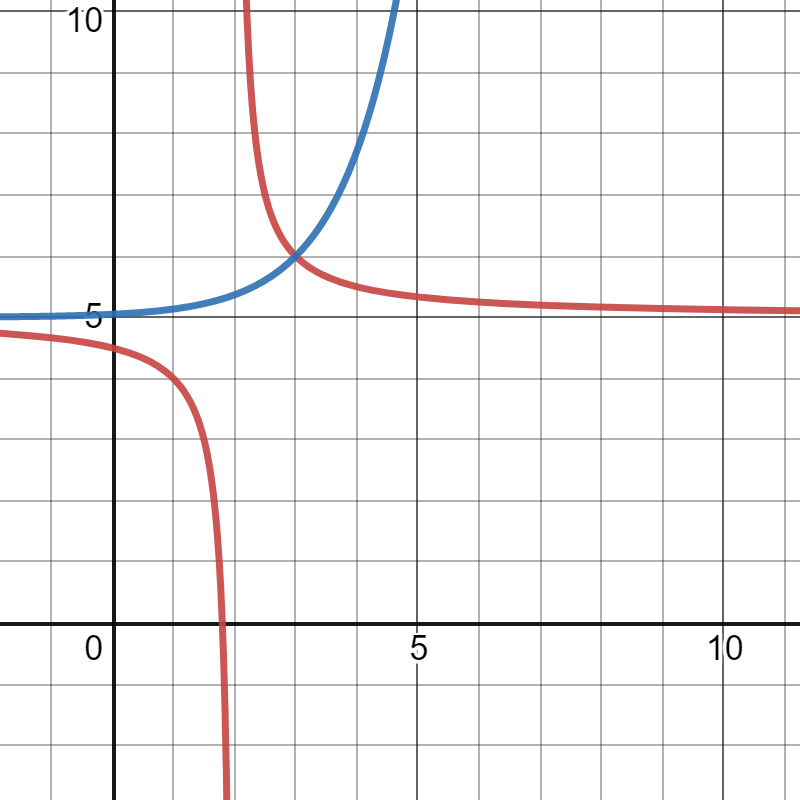
\includegraphics[width=6cm]{desmos ex5.png}
    \end{center}
    \begin{itemize}[<+->]
        \item $(P^{*},Q^{*})=(6,3)$
    \end{itemize}
\end{frame}

\begin{frame}{Exercise 6}
    \begin{itemize}
        \item Suppose supply and demand are given by
        \begin{align*}
            S: Q=\frac{1}{2}P\\
            D: \frac{1}{2}P+Q=12
        \end{align*}
        Find the market equilibrium 
        \item Suppose that Demand shifts left by 4 units. Find the new equation representing demand, and find the new market equilibrium
    \end{itemize}
\end{frame}

\begin{frame}{Solution 6}
    \begin{itemize}[<+->]
        \item Supply and demand are given by
        \begin{align*}
            S: P=2Q\\
            D: P=-2Q+24
        \end{align*}
        and the new Demand equation is given by $P=-2(Q+4)+24=-2Q+16$
        \item Use desmos to check your answers
    \end{itemize}
\end{frame}


\begin{frame}{Comments}
    \begin{itemize}[<+->]
        \item Make sure you are on top of your algebraic knowledge
        \item If the non-linear examples were tough, that is fine: our main focus will be linear examples 
        \item That being said, any of these and more are fair game on a test
    \end{itemize}
\end{frame}

\end{document}